\section{Plasma Properties}
\begin{frame}{Tokamak Plasma}
    The typical plasma in tokamak has the following properties:
    \begin{figure}
        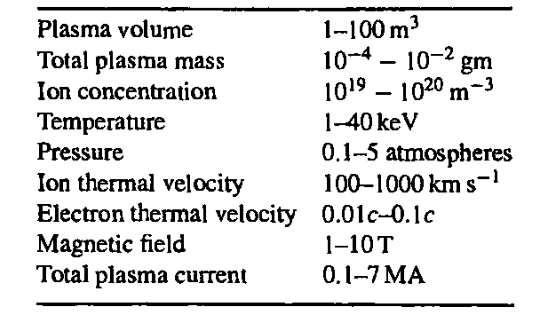
\includegraphics[width=0.7\textwidth]{figures/tokamak-plasma.png}
        \caption{Typical tokamak plasmas}
        \label{fig:typical-tokamak-plasmas}
    \end{figure}
\end{frame}

\begin{frame}{Debye Shielding}
    Due to the high mobility of electrons, the electric field from heavy ions will be shielded by electron cloud. The electric field is very small at certain distance away from ions. Hence, the plasma is quasineutral.

    The number density of ion and electron obey the Boltzmann distribution,
    \begin{equation}
        n_j = n_0 \exp(-\frac{e_j\phi}{T})
        \label{eq:boltzmann-distribution}
    \end{equation}
    The electric potential from an ion shielded by electrons is given by,
    \begin{equation}
        \phi = \frac{e}{4\pi\epsilon_0r} \exp(-\frac{\sqrt{2}r}{\lambda_D})
        \label{eq:electric-potential}
    \end{equation}
    where $\lambda_D$ is the Debye length and is defined by
    \begin{equation}
        \lambda_D = \left(\frac{\epsilon_0 T}{ne^2}\right)^2 = 2.35\times10^5\left(\frac{T}{n}\right)^2
        \label{eq:bebye-length}
    \end{equation}
\end{frame}

\begin{frame}{Plasma Frequency}
    If we pin ions as a static and uniform background, and perturb electrons, then electrons will oscillate around the static ions. The oscillation frequency is called electron plasma frequency, and is
    \begin{equation}
        \omega_{pe} = \left(\frac{ne^2}{\epsilon_0m_e}\right)^{1/2}
        \label{eq:electron-plasma-frequency}
    \end{equation}
    Similarly, the ion plasma has its oscillation frequency as well,
    \begin{equation}
        \omega_{pi} = \left(\frac{ne_i^2}{\epsilon_0m_i}\right)^{1/2}
        \label{eq:electron-plasma-frequency}
    \end{equation}
    where $e_i$ is the charge of ion.
\end{frame}